\documentclass[11pt,oneside,letterpaper]{article}

% graphicx package, useful for including eps and pdf graphics
\usepackage{graphicx}
\DeclareGraphicsExtensions{.pdf,.png,.jpg}

% basic packages
\usepackage{color} 
\usepackage{parskip}
\usepackage{float}

% text layout
\usepackage{geometry}
\geometry{textwidth=15cm} % 15.25cm for single-space, 16.25cm for double-space
\geometry{textheight=22cm} % 22cm for single-space, 22.5cm for double-space

% helps to keep figures from being orphaned on a page by themselves
\renewcommand{\topfraction}{0.85}
\renewcommand{\textfraction}{0.1}

% bold the 'Figure #' in the caption and separate it with a period
% Captions will be left justified
\usepackage[labelfont=bf,labelsep=period,font=small]{caption}

% review layout with double-spacing
%\usepackage{setspace} 
%\doublespacing
%\captionsetup{labelfont=bf,labelsep=period,font=doublespacing}

% cite package, to clean up citations in the main text. Do not remove.
\usepackage{cite}
%\renewcommand\citeleft{(}
%\renewcommand\citeright{)}
%\renewcommand\citeform[1]{\textsl{#1}}

% Remove brackets from numbering in list of References
\renewcommand\refname{\large References}
\makeatletter
\renewcommand{\@biblabel}[1]{\quad#1.}
\makeatother

\usepackage{authblk}
\renewcommand\Authands{ \& }
\renewcommand\Authfont{\normalsize \bf}
\renewcommand\Affilfont{\small \normalfont}

% comments
\usepackage{ulem}
\definecolor{purple}{rgb}{0.459,0.109,0.538}
\def\tb#1#2{\sout{#1} \textcolor{purple}{#2}} 
\def\tbc#1{\textcolor{purple}{[#1]}}



%%% TITLE %%%
\title{\vspace{1.0cm} \LARGE \bf fluB}

\author[1]{Gytis Dudas}
\author[1]{Trevor Bedford}
\author[1]{Samantha Lycett}
\author[1,2]{Andrew Rambaut}

\affil[1]{Institute of Evolutionary Biology, University of Edinburgh, Edinburgh, UK}
\affil[2]{Fogarty International Center, National Institutes of Health, Bethesda, MD, USA.}

\date{\today}

\begin{document}
\maketitle

\begin{abstract}

Influenza B viruses are increasingly being recognized as major contributors to morbidity attributed to seasonal influenza. 
Currently circulating influenza B isolates are known to belong to two antigenically distinct lineages (referred to as B/Victoria and B/Yamagata subtypes (comment - is subtype okay to use here?)) on the basis of haemagglutinin inhibition (HI) assays. 
Frequent reassortment between the segments of these two lineages has been noted in the past (comment - cite Lindstrom et al 1999), but the effects of these reassortments have not been investigated in much detail.

\end{abstract}

\pagebreak


\section*{Introduction}
Seasonal influenza causes an estimated 250,000 to 500,000 deaths annually and is comprised of three species (influenza A, B and C) co-circulating in humans.
Most of these are attributed to influenza A viruses, which are considered to cause the most morbidity and mortality attributed to seasonal influenza.
Though lacking the antigenic diversity that influenza A viruses possess, influenza B viruses are increasingly being recognized as important human pathogens \cite{paul-glezen2013}.
Following the 2009 A/H1N1 pandemic influenza B viruses have circulated more widely than previously (note - reword this) and in the 2012/2013 influenza season in Europe as many as 53\% of influenza sentinel surveillance samples tested positive for influenza B \cite{ECDC1213}. 

Like all members of \textit{Orthomyxoviridae}, influenza B viruses have segmented genomes, which allow viruses co-infecting the same cell to exchange segments (a process known as reassortment). 
Influenza A viruses are widely considered to be a major threat to human health worldwide due to the ability to cause pandemics in humans via reassortment of seasonal human and non-human influenza A strains. 
The only known persistent source of influenza B viruses are humans (and occasionaly seals \cite{osterhaus2000}) and thus the antigenic diversity of influenza B viruses circulating in humans is considered to be low. 
It has been suggested that influenza B viruses use a combination of reassortment and amino acid insertion-deletions to generate antigenic diversity (comment - citation).

Currently circulating influenza B viruses are comprised of two antigenically distinct lineages - Victoria and Yamagata (referred to as Vic and Yam, respectively) which are named after two strains: B/Victoria/02/87 and B/Yamagata/16/88, respectively, which possess antigenically distinct haemagglutinin (HA) surface glycoproteins. 
The two HA lineages still co-circulate today and are thought to have shared a most recent common ancestor in xxxx. 
All other influenza B segments also show a split in xxxx (comment - our estimate \textit{circa} 1984 figure \ref{TMRCAhpd}, use a figure to show TMRCAs and rates for each segment?), although the numbers of strains falling on either side of the split are different due to reassortments following the initial split of Yamagata and Victoria lineages in all segments.

%\begin{figure}[h]
%	\centering		
%	\includegraphics[width=0.95\textwidth]{figures/InfBtmrcaHPD}
%	\caption{\textbf{Provisional TMRCA plot.}}
%	\label{TMRCAhpd}
%\end{figure}

Previously, through the use of time-stamped phylogenetic trees, the complete history of influenza B reassortment events has been reconstructed (comment - cite Chen \& Holmes 2008), and showed extensive and often complicated patterns of reassortment between all segments of influenza B viruses both between and within Vic and Yam lineages.
Another approach exists, however, whereby belonging to either the Victoria or Yamagata lineage in the tree of one segment can be used as a discrete trait in trees of other segments.
Reassortment events which result in the replacement of one segment lineage by another show up as changes in the discrete trait along a branch and allow the inference of parameters related to the subtree descended from the node displaying a changed trait.
Here, we use discrete traits to model inter-lineage reassortments between Victoria and Yamagata lineage segments in BEAST to look at lineage persistence times following reassortment events. 
We show that despite extensive reassortment, PB1, PB2 and HA segments of influenza B viruses still survive as Victoria and Yamagata lineages, which appear to be co-adapted to the point where virions which do not contain PB1, PB2 or HA segments derived entirely from either the Victoria or the Yamagata lineage are selected against.
In other segments (PA, NP, NA, MP and NS) a single lineage has been fixed in the influenza B population: Yam for PA, NP, NA and MP and Vic for NS.


\section*{Methods}

\subsection*{Sequences and subtyping}
We compiled a dataset of 452 complete influenza B genomes from GISAID (comment - need acknowledgment tables). 
Each strain was assigned to a lineage (either Vic or Yam) in each segment by making maximum likelihood trees and looking whether it fell within the subtree containing B/Victoria/02/87 or B/Yamagata/16/88 sequences with the exception of the NS segment (B/Victoria/02/87 was a reassortant and possessed a Yam lineage NS), where B/Norway/1/84 (comment - B/Czechoslovakia/69/1990 could be used as well, since it is the only strain showing an entirely Vic genome) was considered as being representative of Victoria lineage.
Each strain was thus assigned 8 lineages depending on the combination of lineages it belongs to in all trees (for example all segments except for NS in strain B/Victoria/02/87 belong to Vic lineage and can thus be represented as V,V,V,V,V,V,V,Y). 
Seven of these where then used as discrete states in each of the trees (e.g. PB1 tree had PB2, PA, HA, NP, NA, MP and NS as traits and V or Y as trait values) in BEAST (comment - reference BEAST).

\subsection*{Building trees}
For each segment it was attempted to make 3 replicates with 200 million MCMC states (comment - only third replicates ran for that long) each under the HKY model of nucleotide substitutions, 3 codon partitions, robust counting (comment - reference robust counting)) under the GMRF Bayesian skyride demographic model (comment - reference skyride).
In addition we used "relaxed" tips for 94 sequences (of which 93 only had year of isolation and 1 had only year and month of isolation).
We inferred the ancestral state of lineages in each segment by using discrete traits (asymmetric CTMC matrix with BSSVS (comment - cite Philippe)). Because the posterior set of trees have branches labelled with the inferred lineage in all other segments, we can detect inter-lineage reassortments whenever a trait transition is observed (i.e. Y to V or V to Y) between a node and its descendant in any segment. 
In addition, by reconstructing the ancestral state of all other genomic segments jointly we can infer co-reassortment events when more than one trait transition occurs on the same node in a tree.

We use a measure of persistence which is defined as the ratio of distances (in units of time) between a reassortant node and its most recent tip (the event is sampled uniformly over the branch displaying a trait value that is different from its parent node) and compare it to the mean of distances between all nodes and their respective most recent tips. 
If this statistic is below 1 a reassortment event is presumed to be disadvantageous, if it is above 1 the event is presumed to be advantageous.

Alternative - we start by allocating the tips in the tree to yearly bins starting from 1984 and ending in 2013. 

At each state of the MCMC chain we choose a random tip from each bin and traverse the tree towards the root until a reassortment event (i.e. a trait switch) is encountered.
We log the traits which have transitioned at the reassortant node (i.e. the reassorting segment), the direction of transition (e.g. whether the parental node was V and the child node Y or vice versa) and the amount of time separating the tip and the node displaying a trait transition. 
The time taken to traverse back to a reassortment event is expected to be longer for advantageous reassortments than for non-advantageous reassortments.


\subsection*{Building a consensus set of reassortment events}
Maximum clade credibility trees were made after discarding the first 1000 trees as burnin. 
Nodes with trait values different from the trait value of their parental node were classified as being reassortants.
The persistence time, descendant tips and reassorting segments were logged for each reassortant node and aggregated across analyses based on descendant tips.


\subsection*{Measures of diversity}
We inferred the diversity of each segment over time by finding the oldest most recent common ancestor of all branches existing at yearly intervals, which places an upper boundary on diversity existing at each time period.
In addition, we calculated mean pairwise diversity and mean pairwise TMRCA between branches inferred to be in virions possessing Victoria and Yamagata lineage PB1, PB2 and HA.



\subsection*{Work in progress}
Currently running "null" traited trees where trait maps have been rearranged (keeping the same ratio of trait values).


\section*{Results}

\subsection*{PA, NP, NA, MP and NS have periodically lost diversity}
From TMRCA plots (see Figure \ref{tmrcaOT}) it is clear that diversity in PB1, PB2 and HA has been maintained since the initial split of Victoria and Yamagata lineages, whereas other segments (most notably NS) have repeatedly lost lineages.
The plot shows the initial losses of diversity in PA, NP and MP segments in 1997 (x axis), indicative of the extinction of Victoria lineages of those segments and revealing that a reassortment had occured which meant that all sampled lineages circulating around 1997 shared a common ancestor around the year 1990 (y axis).
By 2001, the Yamagata lineage of the NS segment had gone extinct as well, revealing that NS too had reassorted together with PA, NP and MP segment around the year 1990 (similar TMRCA along the y axis to previous reassortants).
Another round of reassortment-related extinction took place since then in PA, MP and NA segments and another 3 in the NS segment.
Unlike all other segments, however, all lineages of PB1, PB2 and HA segments have maintained diversity and lineages circulating in 2011 were still derived from the original split of the Victoria and Yamagata lineages.

These differences in segment diversity are reflected in ratios of Victoria to Yamagata lineages in different segments: for the PB1, PB2 and HA segments the ratio of sequences belonging to either Victoria or Yamagata lineages are close to 0.5 (see Figure \ref{lineageRatios}, whereas all other segments are heavily skewed towards Yamagata lineage with the exception of NS segment which has more Victoria lineage sequences.

\begin{figure}[h]
	\centering		
	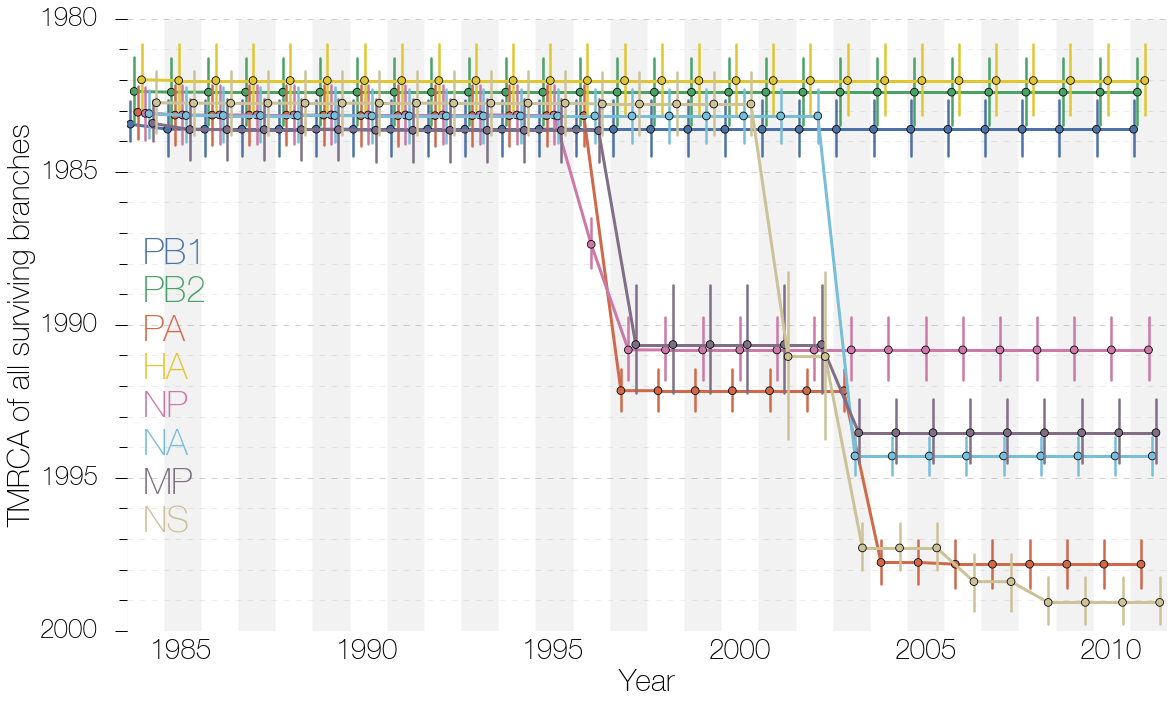
\includegraphics[width=0.95\textwidth]{figures/InfB_tmrcaOT_lines.png}
	\caption{\textbf{TMRCA over time plot.}}
	\label{tmrcaOT}
\end{figure}


\begin{figure}[h]
	\centering		
	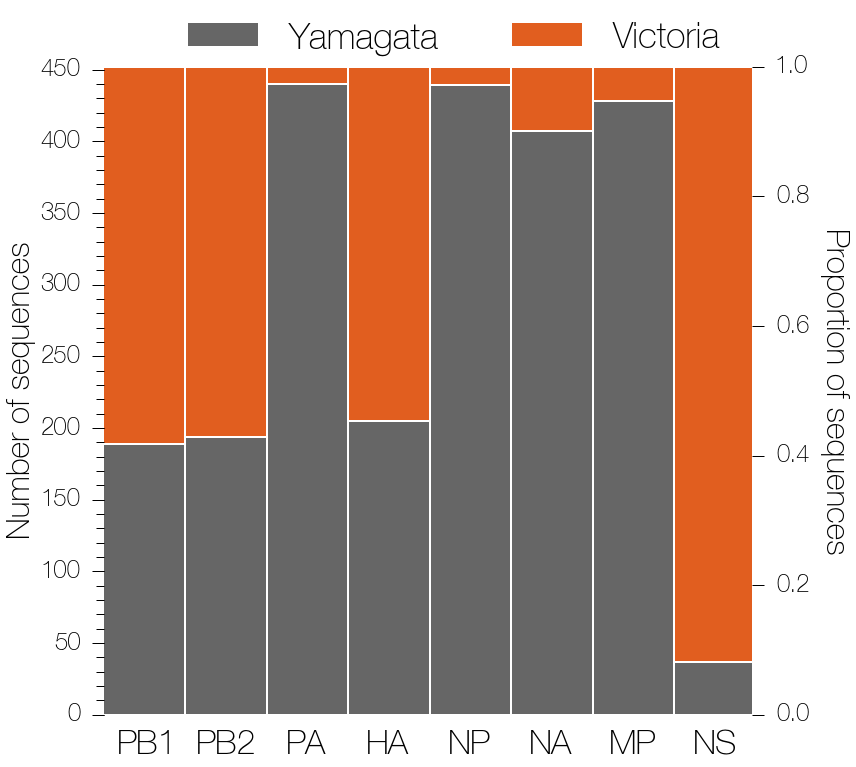
\includegraphics[width=0.95\textwidth]{figures/InfB_LineageRatios.png}
	\caption{\textbf{Ratio of lineages in the dataset.}}
	\label{lineageRatios}
\end{figure}

\subsection*{Diversity in PB1, PB2 and HA segments is not maintained independently}
We find that the diversity preserved in PB1, PB2 and HA segments is not preserved independently in each segment.
Plot XXXX (comment - make date-spectrum figure) shows the posterior distributions of inferred dates of reassortment.
Following 1993 PB1, PB2 and HA reassortments are inferred to occur simultaneously at the same nodes.


\subsection*{Numbers of reassortments and their persistence}

(comment - this bit is for stratified REPU results)
We find that on average, inter-lineage reassortments are common (number of trait switches observed: 116 after filtering, but some will be the same event, naive underestimate is 14.5 inter-lineage reassortments per segment) and favoured by natural selection (persistence statistic > 1, see Figure \ref{stratifiedREPUgraph} (comment - make figure prettier)), although this varies by segments involved and date of reassorment.

In particular, reassortment events where same-lineage PB1, PB2 and HA segments reassort together have much better persistence than events where they reassort independently.
Conversely, reassortments that produce mixed-lineage PB1-PB2-HA complexes have persistence statistic lower than an average node existing at the same time, with the exception of NS.
We see reassortment events preserving the Victoria lineage PB1-PB2-HA complex occuring between 1990 and 1995 in PA, NP and MP (comment - if NS trees were better, there would be a PB1-PB2-HA preserving event in NS segment), coresponding to the origins of the reassortant lineage that eventually gave rise to B/Hong Kong/330/2001-like influenza B viruses, which were the first Victoria lineage HA-bearing viruses detected outside of Asia since 1990s (comment - cite paper).
However, the persistence of segment lineages comprising these B/Hong Kong/330/2001-like reassortant viruses vary dramatically.
Whereas the PA and MP lineages that were part of the reassortant B/Hong Kong/330/2001-like constellation had poor persistence, the NP lineage was "re-used" during the next inter-lineage reassortment occuring around 2000.

The reassortment event occuring around the year 2000 (which produced B/Iowa/03/2002-like viruses), involved the PA, NA, MP and NS segments of Yamagata lineage reassorting with Victoria lineage PB1, PB2 and HA (the latter virus already contained a Yamagata lineage NP) with good persistence (over 2 times the persistence of all other nodes existing at the time).
The greater persistence of PA, NA, MP and NS lineages is due to having left descendants close to the present (essentially becoming the "trunk" lineages of those segments).

Additional reassortments occured in 2004 and 2006.
In 2004 NP, MP and NS segments of Yamagata lineage reassorted with Victoria lineage PB1, PB2 and HA (with Yamagata lineage PA and NA).
This event is one of the most interesting ones, since the NS segment of Victoria lineage PB1-PB2-HA complex, though ancestrally derived from Victoria lineage, was replaced by a Victoria lineage NS segment which had been evolving together with genome constellations derived from Yamagata lineage segments.
Although the MP segment lineage reassorted in the 2004 event eventually became the "trunk" of all Victoria PB1-PB2-HA lineage bearing viruses, the NP(Yam) lineage was replaced by another one (also Yam) that was reassorted into the PB1-PB2-HA Victoria lineage-bearing background in 2006.

From reassortment event persistence times it is clear that reassortment events that break up the PB1-PB2-HA complex have occured in the past but never persisted for long.
We observe a sudden stop of PB1-PB2-HA complex-separating reassortment events after 1995 which are followed solely by PB1-PB2-HA complex-preserving reassortment events.

(comment - this bit is for the tip descent method)
On average it takes nearly 2 years longer for a random tip at any given point to trace its ancestry to a reassortant lineage where a PB1, PB2 and HA segments of the same lineage have reassorted together, although this varies by segment and time of reassortment.


\subsection*{Differentation of segments along PB1, PB2 and HA lineages}
(comment - this will be referring to 3 plots, which are mean pairwise tmrcas between branches under PB1, PB2 and HA traits, respectively)

When comparing TMRCAs between branches of segment trees inferred to be under either Victoria or Yamagata lineage PB1, PB2 or HA, it is clear that diversity along the lineage axis has been preserved in PB1, PB2 and HA, whereas all other segments (PA, NP, NA, MP and NS) have repeatedly lost diversity, indicating reassortments with PB1, PB2 and HA segments.
Interestingly, the diversity patterns between segments under inferred PB1, PB2 or HA lineages differ early on and this can be shown to be due to short lived reassortants with mixed-lineage PB1, PB2 and HA segments, namely the VVY (B/Bankok/163/1990-like), YVV (B/Nanchang/630/1994-like) and YVY (B/New York/24/1993-like) reassortants (comment - will require trees in supplementary info).
Starting from about 1993, however, PB1, PB2 and HA segments of Victoria lineage have only reassorted as one with other segments of Yamagata lineage which is reflected in plots becoming identical, regardless of segment, post-1993.


\section*{Discussion}

\subsection*{Limitations of current study}
The methods used in this paper have limited power to detect reassortments, since lineages have been fixed over time and thus all viruses eventually come to bear either Vic or Yam lineage PA, NP, NA, MP and NS segments.
We can also only detect reassortment events where a lineage has switched from Vic to Yam or \textit{vice versa}, but not when a lineage has switched from a Yam lineage to another Yam lineage, which has occurred in the past (e.g. the 2004 Vic lineage PB1-PB2-HA complex reassortment with NP is only visible in the NP tree, since all viruses in our dataset from 1995 onwards, including Vic PB1-PB2-HA complex-bearing ones, had a Yamagata lineage-derived NP).


\subsection*{Reassortment in influenza B is common and extensive}
Extensive reassortment has long been established as a major pathway by which influenza B viruses generate diversity.
Even focusing on a specific subset of reassortments (those that occur between two lineages and those where the previous lineage was of the opposite lineage) reveals 116 events and if we naively assume that all events are replicated across all trees it still means there have been over 14 inter-lineage reassortment events.
We also see that reassortments occur across considerable phylogenetic distances and some segment lineages have been so successful as part of reassortant viruses that they out-competed their sister lineages (e.g. Yamagata lineages of PA, NP, MP and NA segments). (comment - could include diversity over time plots to show maximum phylogenetic distance attained prior to reassortment for each segment)


\subsection*{Selection maintains the diversity in PB1-PB2-HA complexes of Victoria and Yamagata lineages}
Rather surprisingly, 3 segments have maintained a ratio of Vic and Yam lineages very close to 0.5 (PB1, PB2 and HA) (see Figure \ref{lineageRatios}) and have preserved the diversity that has accumulated since the split of the two lineages (see Figure \ref{tmrcaOT}).
Our results suggest that this is due to the 3 segments co-reassorting (comment - refer to posterior distributions of reassortant dates plot).
We find evidence that this co-reassortment pattern between PB1, PB2 and HA is not due to skewed reassortment ((comment - add Marshall et al 2013 citation) have shown that reassortment efficiency is high in influenza A), but rather due to viruses bearing mixed-lineage PB1-PB2-HA complex having lower fitness than viruses with PB1-PB2-HA complexes derived entirely from Yam or Vic lineages (comment - refer to stratified REPU plot).
Not only are events that split up pure-lineage PB1-PB2-HA complexes rare, but they also have poor persistence and trees have spent less than 10\% of the time in the mixed-lineage PB1-PB2-HA complex state, suggesting that they are selected against (comment - make plot of that).

Thus our findings suggest that the link maintaining PB1, PB2 and HA lineages close to equilibrium is not due to biased reassortment, but a result of selection acting upon reassortants containing mixed-lineage PB1-PB2-HA segments.
We find that by 1995 sufficient co-dependence had developed between PB1, PB2 and HA segments of Victoria and Yamagata lineages to prevent reassortant progeny containing mixed-lineage PB1-PB2-HA complexes from infecting sufficient numbers of individuals to cross the detection threshold.

\subsection*{Segments vary in their abilities to reassort and success as part of reassortant viruses}
A rather striking pattern in influenza B evolution is the fact that segments reassorted at the same time can have dramatically different fates.
For example, PA, NP, MP and NS segments of Yamagata lineage were reassorted into Victoria lineage PB1-PB2-HA background in 1994, but of those 4 segments only the NP lineage persisted for a considerable amount of time, being replaced by another NP lineage in 2006, whereas PA was replaced in 2000 and MP together with NS were replaced by different lineages in 2004.
This suggests that most non-PB1, PB2 or HA segments have the capacity to evolve somewhat independently of the rest of the segments present in the same virion.

\subsection*{Interpreting our results}
(comment - this bit is exceedingly unsubstantiated and ramble-y)
Recently the antigenic drift of influenza B viruses has been characterised (comment - cite Bedford et al 2013) and Victoria lineage HA was found to drift nearly twice as fast as Yamagata lineage HA.
A possible explanation for this would be differences in polymerase fidelity: if Victoria lineage polymerase introduced higher mutation rates, this would explain the higher antigenic drift rate seen in Vic lineage HA, but also would suggest that Vic lineage PB1-PB2-HA complex "borrows" segments from Yamagata lineage PB1-PB2-HA complex-bearing viruses and "breaks" them through going over something akin to each segment's error threshold, necessitating another round of reassortment.
However, we find no evidence of differences in nucleotide, synonymous and non-synonymous rates of evolution between branches that were inferred to have been in the same virion as PB1, PB2 or HA segments of Vic or Yam lineages.
Thus we have no evidence to suggest fundamental differences between Vic and Yam lineage PB1-PB2-HA complexes.

Balancing selection would be expected, and does in the malaria parasite, preserve antigenic diversity, but it is unclear if maintenance of PB1-PB2-HA lineages is driven by balancing selection acting to preserve antigenic diversity of HA or the diversity of PB1 and PB2 segments.
Recently (comment - cite Cobbin et al 2013) a similar link has been described in influenza A by XXXX, where the PB1 segment is reassorted more frequently than expected during vaccine strain creation.
If influenza B virus PB1 has a similar gene-regulatory activity, then it would be reasonable to assume that HA and PB1 are associated through the necessity for HA to have appropriate levels of expression and PB2 hitchhikes together with PB1 due to some functional requirement as part of the polymerase complex.
This does not explain why the Vic lineage of the PA segment was lost so readily, however, despite it being a part of the polymerase complex.

\subsection*{Future evolution of influenza B viruses}
From our current findings it is difficult to extropolate what reassortants will come to dominate the influenza B population in the far future.
It seems likely that PB1, PB2 and HA segments of both Victoria and Yamagata lineages will either continue to co-exist in their co-adapted state or one lineage will go extinct.
Until the 2004 and 2006 reassortment events it seemed like the NP segment would follow the PB1-PB2-HA complex in becoming the next segment to be recruited as part of a co-adapted segment complex.
This method of gradually recruiting more segments to a co-adapted segment complex could have lead to the eventual speciation of influenza B into originally Vic and Yam lineage HA bearing species.
As it stands now, however, the most diversity between Victoria and Yamgata PB1-PB2-HA lineage-bearing viruses has been built up in PA and NA segments (which shared a common ancestor around 2000) and it remains to be seen whether this diversity will too be lost following a reassortment event.

Given the evolutionary history of the NP segment, it would be reasonable to focus sequencing efforts on complete influenza B genome sequencing.
Our results indicate that successful reassortants are likely to come from the combination of Victoria lineage PB1-PB2-HA complex and PA, NP, NA and MP segments of Yamagata lineage (or NS segment of Vic lineage), though the number of Yamagata lineage segments can vary.
It is also obvious that increased surveillance efforts will inevitably uncover a lot of reassortant viruses (possibly even viruses with mixed-lineage PB1-PB2-HA complexes) and the threshold at which these reassortants should be considered as being likely to take over the influenza B population would require further work.

\subsection*{Testing the co-dependence between PB1, PB2 and HA segments}
Our results suggest a simple test for the hypothesis that PB1, PB2 and HA segments of Victoria and Yamagata lineages have become co-dependent - if PB1, PB2 or HA segments from different lineages were combined artificially in a single virion, these should have lower fitness than virions containing wholly Victoria or wholly Yamagata lineage PB1-PB2-HA complex.
We also expect that the fitness of artificially derived reassortants would decline with increasing date of strain isolation i.e. mixed-lineage PB1-PB2-HA containing reassortants with segments from older isolates having higher fitness than reassortants possessing segments of more recent isolates.

\subsection*{Implications for influenza B surveillance and prevention}
The findings presented here have several implications.
On one hand, if the co-dependence between PB1, PB2 and HA segments is strong enough, influenza B viruses containing mixed-lineage PB1-PB2-HA complex detected by surveillance are unlikely to contribute to long-term evolution of influenza B viruses.
On the other hand, the dependence of the HA segment on PB1 and PB2 segments (or vice versa) implies that more subtle disease control measures can be developed and used against influenza B viruses.
Finally, the extent of inter-lineage reassortment argues for more extensive surveillance of influenza B viruses, as sequences of a handful of segments will not necessarily tell the whole story, especially since influenza B viruses have been known to evolve counter-intuitively (e.g. losing Victoria lineages of PA and NA segments despite their associations with the rest of the polymerase complex or role in antagonising HA activity, respectively).
This study also highlights the gaps in our knowledge of the molecular biology of influenza B viruses.



%\begin{figure}[h]
%	\centering		
%	\includegraphics[width=0.95\textwidth]{figures/InfB_TMRCAOverTime}
%	\caption{\textbf{Provisional TMRCA over time plot.}}
%\end{figure}


\bibliographystyle{plos}
\bibliography{fluB}
\end{document}
